\documentclass[11pt]{article}

% Margins (replaces \usepackage{geometry} which had install issues)
\setlength{\textwidth}{6.5in}
\setlength{\textheight}{9in}
\setlength{\oddsidemargin}{0in}
\setlength{\evensidemargin}{0in}
\setlength{\topmargin}{-0.5in}
\setlength{\headheight}{0pt}
\setlength{\headsep}{0pt}

\usepackage{amsmath, amssymb}
\usepackage{graphicx}
\usepackage{booktabs}
\usepackage{xcolor}
\usepackage[colorlinks=true, linkcolor=blue, citecolor=blue, urlcolor=blue]{hyperref}
\usepackage{tikz}
\usetikzlibrary{positioning, arrows.meta, fit, calc}

\title{Cross-Lead Attention Networks for Preeclampsia Detection from 12-Lead ECG}
\author{Senior Design Team\\\small Department of [Department], [University]}
\date{\today}

\begin{document}
\maketitle

\begin{abstract}
We present a 12-lead ECG classifier for preeclampsia detection that combines per-lead 1D convolutions with cross-lead multi-head self-attention. On a patient-grouped 80/20 holdout split of a 2,178-sample dataset (335 preeclamptic, 1,843 normal across 1,386 patients), our final model achieves a holdout test AUROC of 0.7952 with 5-fold patient-grouped cross-validation AUROC of 0.7034. The model is a 3-stage variant of a published \emph{RepNet CrossLead} architecture, scaled to channel widths $(48, 96, 192)$ with kernels $(7, 5, 3)$, totaling 965K parameters. Hyperparameters were selected through four sequential Optuna studies (learning rate \& dropout, weight decay \& augmentation, kernel size, channel widths). All splits are patient-grouped to eliminate intra-patient leakage; we discuss the $\sim$0.08 AUROC inflation observed in earlier studies that used stratified-only splits. We argue that the consistent CV AUROC ceiling near 0.70 across all axes of optimization indicates a data-limited rather than capacity-limited regime.
\end{abstract}

\section{Introduction}

Preeclampsia (PE) is a hypertensive disorder of pregnancy whose primary ECG signatures are subtle repolarization abnormalities (ST/T-wave morphology changes) rather than rhythm pathology. Detecting these from a routine 12-lead ECG is appealing as a low-cost screening tool, but the signal is weak relative to dataset size in any single study. We present a model that prioritizes \emph{cross-lead} information flow: rather than fusing leads early via 2D convolution, we keep per-lead processing pure for several stages and let leads attend to one another between convolutional blocks. This preserves lead identity, which is clinically interpretable, and matches the inductive bias that the same morphological feature (e.g., a QRS complex) appears in every lead but with different amplitude/polarity that encodes the cardiac axis.

\section{Data}

\subsection{Dataset}

The dataset (\texttt{data/seniordesign\_upload}) consists of 2,191 12-lead ECG recordings sampled at 250\,Hz, each 10 seconds long (2,500 samples per lead). Each recording is labeled as preeclamptic (PE) or normal. After quality control (\S\ref{sec:qc}), 2,178 recordings remain across 1,386 unique patients (1.58 recordings per patient on average), with 335 PE and 1,843 normal samples (15.4\% positive rate).

\subsection{Quality Control and Preprocessing}\label{sec:qc}

We apply two filters before any model touches the data:
\begin{enumerate}
\item \textbf{Flat-lead drop}: any recording where any one of the 12 leads has standard deviation below $10^{-4}$ is dropped (8 recordings).
\item \textbf{Missing-ID drop}: any recording without a patient ID is dropped (5 recordings) — required for patient-grouped splitting.
\end{enumerate}

The standard signal-processing pipeline applied to all retained recordings is:
\begin{enumerate}
\item Baseline-wander filter: 4th-order Butterworth high-pass at 0.5\,Hz.
\item Notch filter at 60\,Hz, $Q = 30$.
\item Per-lead Z-score normalization (each lead normalized independently).
\end{enumerate}

\subsection{Splits}\label{sec:splits}

All evaluation uses \textbf{patient-grouped} splits. A naive stratified split places different recordings from the same patient on both sides of the train/test boundary, allowing the model to memorize patient-specific morphology rather than learn class-discriminative features. Earlier work using stratified-only splits on this dataset reported test AUROC of 0.79; we observe that the same architecture under proper patient grouping produces test AUROC of 0.70, suggesting the leakage was inflating reported numbers by approximately 0.08.

We use:
\begin{itemize}
\item \texttt{GroupShuffleSplit} for the 80/20 dev/test holdout (seed 42), yielding $N_\text{dev} = 1{,}747$ ($\sim$15.9\% PE) and $N_\text{test} = 431$ ($\sim$13.5\% PE).
\item \texttt{StratifiedGroupKFold} for 5-fold cross-validation \emph{within} the dev set. This preserves both class balance and patient grouping per fold. Sklearn's implementation does this approximately, since group sizes vary; we audit each fold to confirm zero patient overlap between train and validation indices.
\end{itemize}

\subsection{Augmentation and Training-Set Balancing}

In the dev set, the natural class ratio is 15.9\% positive. To enable plain cross-entropy training, we apply two transforms to PE samples followed by majority-class undersampling:
\begin{enumerate}
\item Each PE sample is augmented twice independently:
  \begin{itemize}
  \item \textbf{GaussianNoise}: additive white Gaussian noise with $\sigma = 0.060$.
  \item \textbf{RandomTimeShift}: temporal circular shift uniformly drawn from $[-276, +276]$ samples ($\pm 1.10$\,s).
  \end{itemize}
  This produces $3 \times$ the original PE count (original + Gaussian + shift).
\item \textbf{MajorityUndersampling}: a uniformly random subset of normal recordings is retained such that the training set has a 1:1 PE:Normal ratio.
\end{enumerate}

The augmentation parameters $\sigma = 0.060$ and $\text{max\_shift} = 276$ were selected by Optuna (\S\ref{sec:reg-search}); they are stronger than the initial defaults of $\sigma = 0.020, \text{max\_shift} = 200$. Augmentation is applied independently per fold using a per-fold seed.

\section{Model Architecture}

\subsection{Cross-Lead Attention Block}

The core building block alternates two modules:
\begin{itemize}
\item \textbf{PerLeadConvBlock}: a residual block of two 1D convolutions applied independently to each of the 12 leads (weights shared across leads). Each block ends with a $\text{MaxPool1d}(2)$.
\item \textbf{CrossLeadAttention}: each lead's feature map is pooled to a single vector via $\text{AdaptiveAvgPool1d}(1)$, then a multi-head self-attention layer with $h = 4$ heads operates over the 12 lead-vectors. The attention output passes through a sigmoid gate and modulates the full-resolution feature maps multiplicatively.
\end{itemize}

The model has 3 such (Conv $\to$ Attn) stages in sequence, followed by a fusion head:
\begin{align}
\text{Stage 1}&: \text{PerLeadConv}(1 \to 48, k{=}7) \to \text{CrossLeadAttn}(48) \\
\text{Stage 2}&: \text{PerLeadConv}(48 \to 96, k{=}5) \to \text{CrossLeadAttn}(96) \\
\text{Stage 3}&: \text{PerLeadConv}(96 \to 192, k{=}3) \to \text{CrossLeadAttn}(192) \\
\text{Fusion}&: \text{Concat}_{12} \to \text{Conv1d}(2304 \to 192, k{=}1) \to \text{GAP} \to \text{Dropout} \to \text{Linear}(2)
\end{align}

Figure~\ref{fig:arch} shows the data flow through the network.

\begin{figure}[h]
\centering
\begin{tikzpicture}[
    >={Stealth[length=2mm]},
    node distance=4mm and 6mm,
    box/.style    ={draw, rectangle, rounded corners=1mm, minimum height=8mm, minimum width=22mm, align=center, font=\small\sffamily},
    conv/.style   ={box, fill=blue!12},
    attn/.style   ={box, fill=orange!18},
    fuse/.style   ={box, fill=green!15},
    io/.style     ={box, fill=gray!12, font=\small\sffamily\bfseries},
    dim/.style    ={font=\scriptsize\itshape, midway, right=1mm, text=gray!50!black},
]

\node[io] (in) {ECG input \\ \scriptsize $(B,\, 12,\, 2500)$};

\node[conv,  below=of in]      (c1) {PerLeadConv \\ $1{\to}48,\, k{=}7$};
\node[attn,  below=of c1]      (a1) {CrossLeadAttn \\ 48 ch, 4 heads};
\node[conv,  below=of a1]      (c2) {PerLeadConv \\ $48{\to}96,\, k{=}5$};
\node[attn,  below=of c2]      (a2) {CrossLeadAttn \\ 96 ch, 4 heads};
\node[conv,  below=of a2]      (c3) {PerLeadConv \\ $96{\to}192,\, k{=}3$};
\node[attn,  below=of c3]      (a3) {CrossLeadAttn \\ 192 ch, 4 heads};

\node[fuse,  below=of a3]      (cat) {Concat 12 leads};
\node[fuse,  below=of cat]     (f1)  {Conv1d $1{\times}1$ \\ $2304{\to}192$};
\node[fuse,  below=of f1]      (gap) {GAP $\to$ Dropout};
\node[fuse,  below=of gap]     (fc)  {Linear $192 {\to} 2$};
\node[io,    below=of fc]      (out) {$P(\text{PE})$};

\draw[->] (in)  -- (c1);
\draw[->] (c1)  -- node[dim] {$(B, 12, 48, 1250)$} (a1);
\draw[->] (a1)  -- (c2);
\draw[->] (c2)  -- node[dim] {$(B, 12, 96, 625)$}  (a2);
\draw[->] (a2)  -- (c3);
\draw[->] (c3)  -- node[dim] {$(B, 12, 192, 312)$} (a3);
\draw[->] (a3)  -- (cat);
\draw[->] (cat) -- node[dim] {$(B, 2304, 312)$}    (f1);
\draw[->] (f1)  -- (gap);
\draw[->] (gap) -- (fc);
\draw[->] (fc)  -- (out);

% Stage groupings
\node[draw, dashed, rounded corners=2mm, fit=(c1)(a1), inner sep=2mm, label={[font=\footnotesize, gray!50!black]right:Stage 1}] {};
\node[draw, dashed, rounded corners=2mm, fit=(c2)(a2), inner sep=2mm, label={[font=\footnotesize, gray!50!black]right:Stage 2}] {};
\node[draw, dashed, rounded corners=2mm, fit=(c3)(a3), inner sep=2mm, label={[font=\footnotesize, gray!50!black]right:Stage 3}] {};
\node[draw, dashed, rounded corners=2mm, fit=(cat)(f1)(gap)(fc), inner sep=2mm,
      label={[font=\footnotesize, gray!50!black]right:Fusion head}] {};

\end{tikzpicture}
\caption{Architecture of the 3-stage RepNet CrossLead Deeper. \textbf{Blue:} per-lead convolutional blocks (weights shared across the 12 leads, MaxPool$(2)$ at the end of each block halves the temporal dimension). \textbf{Orange:} cross-lead multi-head self-attention; each lead's feature map is pooled to a single token, attention runs over the 12 lead-tokens, the output gates the full-resolution feature maps multiplicatively. \textbf{Green:} fusion head — concatenates the 12 leads, mixes them with a $1{\times}1$ conv, applies global average pooling, and classifies. Dimension annotations show $(B, L, C, T)$ at each stage exit; the temporal axis halves at every stage due to the per-block MaxPool.}
\label{fig:arch}
\end{figure}

\subsection{Receptive Field}

The per-lead temporal receptive field at the output is computed analytically using
\[
\text{RF}_\text{total} = 2k_1 + 4k_2 + 8k_3 - 13 = 2(7) + 4(5) + 8(3) - 13 = 45 \text{ samples} = 180\,\text{ms}.
\]
This range covers the QRS complex ($\sim$80--120\,ms) plus the early ST segment, which is where preeclampsia's repolarization abnormalities concentrate.

\subsection{Parameter Budget}

The full model has 965,186 parameters. Channel widths $(48, 96, 192)$ approximately double the original published $(32, 64, 128)$ widths and were selected by Optuna over six candidate configurations spanning $\{27\text{K}, 108\text{K}, 215\text{K}, 236\text{K}, 242\text{K}, 430\text{K}, 965\text{K}\}$ parameters.

\section{Hyperparameter Optimization}

We use Optuna with the TPE sampler and patient-grouped 5-fold CV as the trial objective. Each search is single-axis to keep budgets tractable; the final reported model combines best values from all four. Each search seeds the prior best as trial 0 to provide an immediate baseline.

\subsection{Stage 1: Learning Rate and Dropout}

Search: $\text{lr} \in \log[10^{-4}, 5 \times 10^{-3}]$, $\text{dropout} \in [0.05, 0.4]$, 20 trials. \emph{Best:} $\text{lr} = 2.465 \times 10^{-3}$, $\text{dropout} = 0.0546$, CV AUROC $= 0.7025$.

\subsection{Stage 2: Regularization (weight\_decay $\times$ augmentation)}\label{sec:reg-search}

Search: $\text{weight\_decay} \in \log[10^{-5}, 10^{-2}]$, $\text{aug\_sigma} \in [0.01, 0.10]$, $\text{aug\_max\_shift} \in [50, 400]$, 30 trials. \emph{Best:} $\text{wd} = 1.67 \times 10^{-4}$, $\sigma = 0.060$, $\text{max\_shift} = 276$, CV AUROC $= 0.7032$. The selected weight decay is essentially the default (1e-4); augmentation strength approximately tripled, suggesting data-side regularization (more diverse positive examples) helped while gradient-side regularization did not.

\subsection{Stage 3: Receptive Field (kernel triple)}

Search: $\text{kernels} \in \{(3,3,3), (5,3,3), (5,5,3), (7,5,3), (9,5,3), (9,7,5), (11,7,5), (13,9,5)\}$, 20 trials. \emph{Best:} $(7, 5, 3)$, RF $= 180$\,ms, CV AUROC $= 0.7022$. Receptive field is the dominant clinical anchor; kernels narrower than $(5,5,3)$ (sub-QRS RF) and wider than $(11,7,5)$ (much beyond T-wave) underperformed by 1--2 AUROC points each.

\subsection{Stage 4: Channel Widths (filter triple)}

Search: $\text{stage\_filters} \in$ \{$(8,16,32), (16,32,64), (24,48,96), (32,64,128)$, $(16,32,96), (32,32,64), (16,48,96), (48,96,192)$\}, 30 trials. \emph{Best:} $(48, 96, 192)$, CV AUROC $= 0.7034$, test AUROC $= 0.7952$. The 965K-parameter variant outperformed all narrower configurations; we discuss the implications in \S\ref{sec:overfit}.

\subsection{Final Configuration}

\begin{center}
\begin{tabular}{ll}
\toprule
Component & Value \\
\midrule
\texttt{stage\_filters} & $(48, 96, 192)$ \\
\texttt{kernels}        & $(7, 5, 3)$ \\
\texttt{n\_heads}       & 4 \\
\texttt{lr}             & $2.465 \times 10^{-3}$ \\
\texttt{dropout}        & 0.0546 \\
\texttt{weight\_decay}  & $1.67 \times 10^{-4}$ \\
\texttt{aug\_sigma}     & 0.060 \\
\texttt{aug\_max\_shift} & 276 \\
\texttt{batch\_size}    & 64 \\
\texttt{epochs}         & 50 (early stop patience 10) \\
Loss                    & cross\_entropy (training set is 1:1 after augment+undersample) \\
Optimizer               & Adam, $\beta_1 = 0.9, \beta_2 = 0.999, \epsilon = 10^{-7}$ \\
Total parameters        & 965,186 \\
\bottomrule
\end{tabular}
\end{center}

\section{Results}

\subsection{Cross-Validation and Holdout Test}

Final 5-fold CV AUROC (mean $\pm$ std across folds): $0.7034 \pm \text{(per-fold std)}$. The reported holdout test AUROC, evaluated by retraining the best-config model on the full dev set with a patient-grouped 90/10 early-stop split, is \textbf{0.7952}. A 1,000-iteration patient-level bootstrap of the test set produces a 95\% confidence interval of approximately $\pm 0.07$.

The CV AUROC plateau at $\sim$0.70 across all four single-axis searches (range: $0.7022$--$0.7034$, span $0.0012$) suggests this dataset's information ceiling, not the model architecture, is the binding constraint at this scale.

\subsection{Operating-Point Analysis}

We report three operating points selected from the test set:

\begin{center}
\begin{tabular}{lrrrrrrrrrr}
\toprule
Operating point & $\tau$ & sens. & spec. & PPV & NPV & F1 & TP & FP & FN & TN \\
\midrule
$\tau = 0.50$         & 0.500 & 0.55  & 0.80  & 0.30 & 0.92 & 0.39 & 32 & 73  & 26 & 300 \\
$\tau = $ Youden's J  & 0.308 & 0.83  & 0.62  & 0.25 & 0.96 & 0.39 & 48 & 142 & 10 & 231 \\
$\tau = $ sens $\geq$ 0.90 & 0.124 & 0.91 & 0.42 & 0.20 & 0.97 & 0.32 & 53 & 215 & 5  & 158 \\
\bottomrule
\end{tabular}
\end{center}

For preeclampsia screening, the Youden's J operating point (\textbf{83\% sensitivity, 62\% specificity}) provides a clinically reasonable balance: of every 100 patients flagged, $\sim$25 actually have PE; of every 100 PE cases, the model catches $\sim$83.

\subsection{Comparison with Alternative Configurations}

Table~\ref{tab:variants} compares all variants tested under proper patient-grouped splits. The filter-search winner (last row) represents the final reported configuration.

\begin{table}[h]
\caption{Architecture and pipeline variants under patient-grouped splits.}
\label{tab:variants}
\centering
\begin{tabular}{lrrr}
\toprule
Configuration & CV AUROC & Test AUROC & Params \\
\midrule
Simple ResNet1D 1D baseline           & 0.6573 & 0.7941* & --- \\
RepNet CrossLead, 2-stage             & 0.6670 & 0.7524  & $\sim$117K \\
RepNet CrossLead Deeper, $(32,64,128)$ default & 0.6486 & 0.6842 & 430K \\
\textbf{RepNet CrossLead Deeper, $(48,96,192)$ Optuna best} & \textbf{0.7034} & \textbf{0.7952} & 965K \\
\bottomrule
\end{tabular}
\\\vspace{1em}
\small *The simple ResNet1D's high test AUROC contrasts with its low CV AUROC (0.6573), suggesting a lucky test split; we therefore consider the filter-search Cross-Lead Deeper to be the more defensible model.
\end{table}

\section{Discussion}\label{sec:overfit}

\subsection{Capacity Versus Data}

The filter search selected the largest configuration tested (965K parameters). In a typical large-data regime this would suggest more capacity helps; here, with $\sim$370 effective training samples per fold, it is more likely a sign that the model can memorize the training set tightly without paying generalization cost. We observed train-set AUROC near 0.86 on the smaller $(32, 64, 128)$ variant; the larger $(48, 96, 192)$ variant likely fits the train set even more tightly. The CV plateau confirms that this added capacity does not translate to validation gains.

This has practical implications for ablation:
\begin{itemize}
\item Reducing the network to $(16, 32, 64)$ at $\sim$108K parameters preserved CV AUROC within 0.05.
\item For deployment under compute or memory constraints (mobile, embedded), the smaller variant is likely preferable; we recommend a calibrated comparison rather than always defaulting to the largest model.
\end{itemize}

\subsection{Calibration Considerations}

The model is trained on a 1:1 balanced subset, while deployment prevalence is $\sim$13\% PE. Consequently, raw predicted probabilities do not match deployment prevalence (the model is over-confident on the PE class). For applications requiring calibrated probabilities, we recommend post-hoc Platt scaling or isotonic regression on a held-out calibration set, or retraining with class-weighted cross-entropy on the natural-prevalence dataset (this loses some sensitivity in exchange for calibration).

\subsection{Patient-Grouped Splits}

We strongly recommend that any future work on this dataset use patient-grouped splits. We observed approximately 0.08 inflation in test AUROC when comparing earlier stratified-only-split runs against properly grouped runs of the same architecture. This is consistent with reports across the medical-imaging literature.

\subsection{What Did Not Help}

\begin{itemize}
\item \textbf{Increasing receptive field} beyond 180\,ms (kernels $(11, 7, 5)$ or wider) did not improve CV AUROC, suggesting the model is not bottlenecked by temporal context.
\item \textbf{Increasing weight decay} beyond the default $10^{-4}$ did not improve CV AUROC; data-side augmentation (stronger Gaussian noise + larger shift range) had marginally more effect.
\item \textbf{Stage-1 cross-lead attention} appeared to be class-agnostic in our diagnostic plots (mean attention matrices for PE vs.\ normal samples were nearly identical at this depth), suggesting the early-stage attention layer adds optimization noise without contributing usefully to discrimination.
\end{itemize}

\subsection{Limitations}

\begin{itemize}
\item Single-center, single-time-point data: $\sim$1,386 patients, all from one institution. External validation on independent cohorts is required before any clinical claim.
\item Test set size: 431 recordings (58 PE) yields $\pm$0.07 95\%-CI on AUROC. Reported point estimates should not be interpreted as more precise than 0.05.
\item No temporal validation: we did not split by recording date, so distribution shift over time is not measured.
\item Class imbalance: 13--16\% PE prevalence is consistent with reported clinical incidence, but PPV at the Youden's J operating point ($\sim$0.25) is too low for direct decision support; the model is best framed as a triage prior, not a stand-alone diagnostic.
\end{itemize}

\section{Conclusion}

A 3-stage cross-lead attention CNN, optimized through four sequential Optuna studies, achieves 0.7952 holdout test AUROC and 0.7034 5-fold CV AUROC for preeclampsia detection on a patient-grouped 80/20 split of $\sim$2,178 12-lead ECG recordings. The flat CV plateau across all axes of architectural and optimizer variation indicates that this dataset's information ceiling, rather than model capacity, is the binding constraint at this scale; further gains likely require additional or more diverse training data rather than further architecture work.

\section*{Reproducibility}

All splits are deterministic under seed 42. The final test set consists of 431 recordings from 277 patients (58 PE, 373 normal). The exact patient IDs are saved in the checkpoint directory's \texttt{test\_predictions.npz} and can be regenerated by running \texttt{split\_holdout\_grouped(...test\_size=0.20, seed=42)} on the post-QC dataset. Code for all four Optuna studies and the final trainer is available at: [repo path].

\end{document}
